\documentclass[10pt]{article}

\usepackage{spheric}
%%%TITLE
\title{An SPH simulation of bubble cavity evolution on underwater movement}
\date{}

%%AFFILIATIONS
\author[1]{Jiaru Shao}
\author[2]{Moubin Liu$^\dagger$}
\affil[1]{College of Mechanical Engineering, Chongqing University of Technology, Chongqing, China}
\affil[2]{College of Engineering, Peking University, Beijing, China}
\affil[$\relax$]{\email{\dagger}{mbliu@pku.edu.cn}}


%%DOCUMENT
\begin{document}

\maketitle

%\SelectedTopics{}

%%PLEASE PUT YOUR ABSTRACT HERE
\begin{abstract}
Bubble cavities are very common in underwater movement problems. When objects move with a relatively high speed, bubble cavities will be generated, and the behaviour of moving objects will also be affected conversely. In this paper, the evolutions of bubble cavities in different cases are studied using smoothed particle hydrodynamics (SPH) method, which has special advantages in modelling free surfaces, moving interfaces and deformable boundaries. Firstly, the effectiveness of SPH method is validated by a water entry example firstly, which obtain similar results with experiment. Then the underwater movement of some objects with different velocities and shapes are researched, and the formation, growth and collapse of the bubble cavities are analyzed. It is found that the velocities, angles and shapes of the moving objects will affect the bubble cavities greatly, and the SPH model can give optimal predication of these corresponding conditions, which can decrease the impact force on the moving bodies sharply.

\begin{figure}[!htb]
\centering
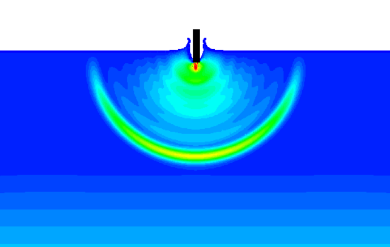
\includegraphics[width=0.3\textwidth]{20-11.png}~~
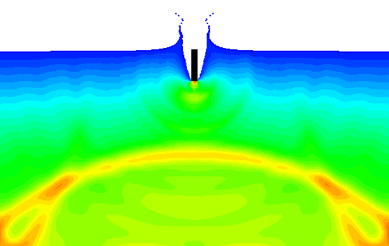
\includegraphics[width=0.3\textwidth]{20-12.png}~~
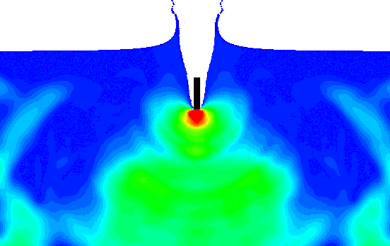
\includegraphics[width=0.3\textwidth]{20-13.png}

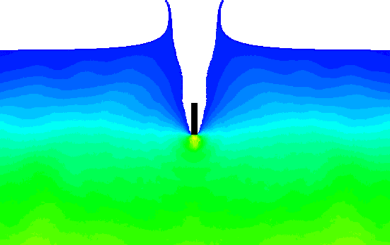
\includegraphics[width=0.3\textwidth]{20-14.png}~~
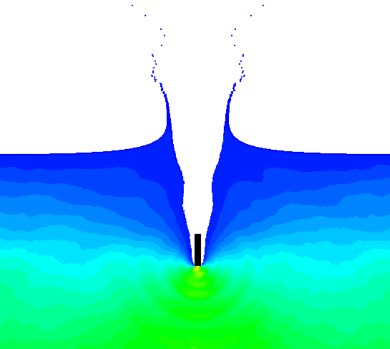
\includegraphics[width=0.3\textwidth]{20-15.png}~~
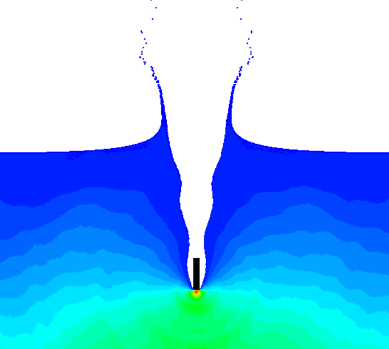
\includegraphics[width=0.3\textwidth]{20-16.png}
\caption{Pressure evolution at 0.01, 0.03, 0.06, 0.09, 0.12, 0.15 s}\label{fig:}
\end{figure}
\end{abstract}


%%THE END OF ABSTRACT

%\addbib

\end{document}
